\section{Uncertainties}
The uncertainty in the measured positions comes from the
precision of alignment of the X-ray device, and resolution of the
rotation angle monitoring instruments. The optical survey used
for the alignment has resolution of 0.1~mm in each coordinate
(x,y,z), which directly affects the Z coordinate of the
measurement. The error in X-ray $\phi$ coordinate due to
misalignment of the X-ray device is not easily evaluated as it
varies with $\phi$.  The maximum deviation over the scanning
$\phi$ range due to variation in (x,y) in the following
combinations is  considered as $\phi$ uncertiainty:
(0,$\pm\sigma_{xy}$),($\pm\sigma_{xy}$,0),
($\pm\sigma_{x}$,$\pm\sigma_{y}$), where $\sigma_{xy} =
\sqrt{\sigma_{x}^{2}+\sigma_{y}^2}$.

The rotation angles about all three axes are monitored using the
laser system as well as the buble-level, and provide Z and $\phi$
dependent corrections to the X-ray coordinates.  The uncertainty
on the x,y rotations come from variation in the recorded laser
intensity.  The corresponding uncertainty in the Z correction is
calculated to be 0.03~mm (6\%), varying with both X-ray
coordinates.  The z rotation is measured by the bubble-level with
0.08~mrad (13\%) uncertainty, defined as maximum deviation in the
measured values at each Z position  over mutiple runs throughout
the data-taking period.  The statistical uncertainty in the
photodetector position is introduced due to fluctuation in the
number of X-ray interactions. The interaction rates are measured
with 10\% precision leading to statistical uncertainty in the
fitted position of  0.11~mm (0.16~mrad).  A summary of all
uncertainties contributing to the measured Z and $\phi$ positions
with 2018 data is given in table~\ref{tab:uncertainties}; similar
results determined with 2017 data are shown.

A measure of overall precision of the measurement can be
estimated using spacing of adjacent MPPC pairs calculated in
table~\ref{tab:oddeven}.  We expect the spacing to be uniform and
infer the precision of the single measurement based on the
standard deviation of the pairwise spacing. Conservatively, the
calculation shows $\sigma_Z$= 0.40~mm and $\sigma_\phi$=
0.56~mrad, higher than expected from the systematic and
statistical sources considered indicating that there are
additional sources of uncertainty which are not included. The
precision, however, is within the experimental goals as well as
the aims of this X-ray survey.

An alternate means of validation of the X-ray measurement is
provided by the lead absorber strips attached to the front face
of the LXe cryostat (fig \ref{fig:lead1}), which can be located
independently by X-ray and optical surveys.  Eight thin strips
(30$\times$3 mm$^2$) are placed lengthwise along $\hat{z}$ or
$\hat{\phi}$ direction each.  Scanning with X-ray shows a deficit
of interactions in the photodetector due to X-ray absorption,
which is fitted with a gaussian shape added to the photodetector
fitting function described in sec.\ref{eqn:mppcfitfcn}.
Comparison of the X-ray and optical survey measurements of strip
positions show good agreement, with standard deviation
$\sigma_Z$= 0.41~mm and $\sigma_\phi$= 0.67~mrad, comparable to
the one observed with MPPC spacing.  The results are included in
table \ref{tab:uncertainties} and shown in figure \ref{fig:lead2}.

\begin{table}
\begin{tabular}{clcc}
 & Source & Z Unc [mm] & $\phi$ Unc [mrad] \\
  \hline
1& Alignment      & 0.1  & 0.21  \\
2& Fit           &  0.11 & 0.16  \\
3& Laser System  &  0.03 &  - \\
4& Bubble-level  &  -    & 0.08 \\
5& MPPC spacing  & 0.40  & 0.56 \\
6& Lead Strip   &  0.41  & 0.67 \\
\end{tabular}
\caption{Summary of uncertainties on the measured photodetector
positions in 2018 X-ray scan. Sources 1-4 show individual
contributions to the measurement, sources 5 and 6 show
total uncertainty measured using two different methods.
}
\label{tab:uncertainties}
\end{table}

\begin{figure}[]
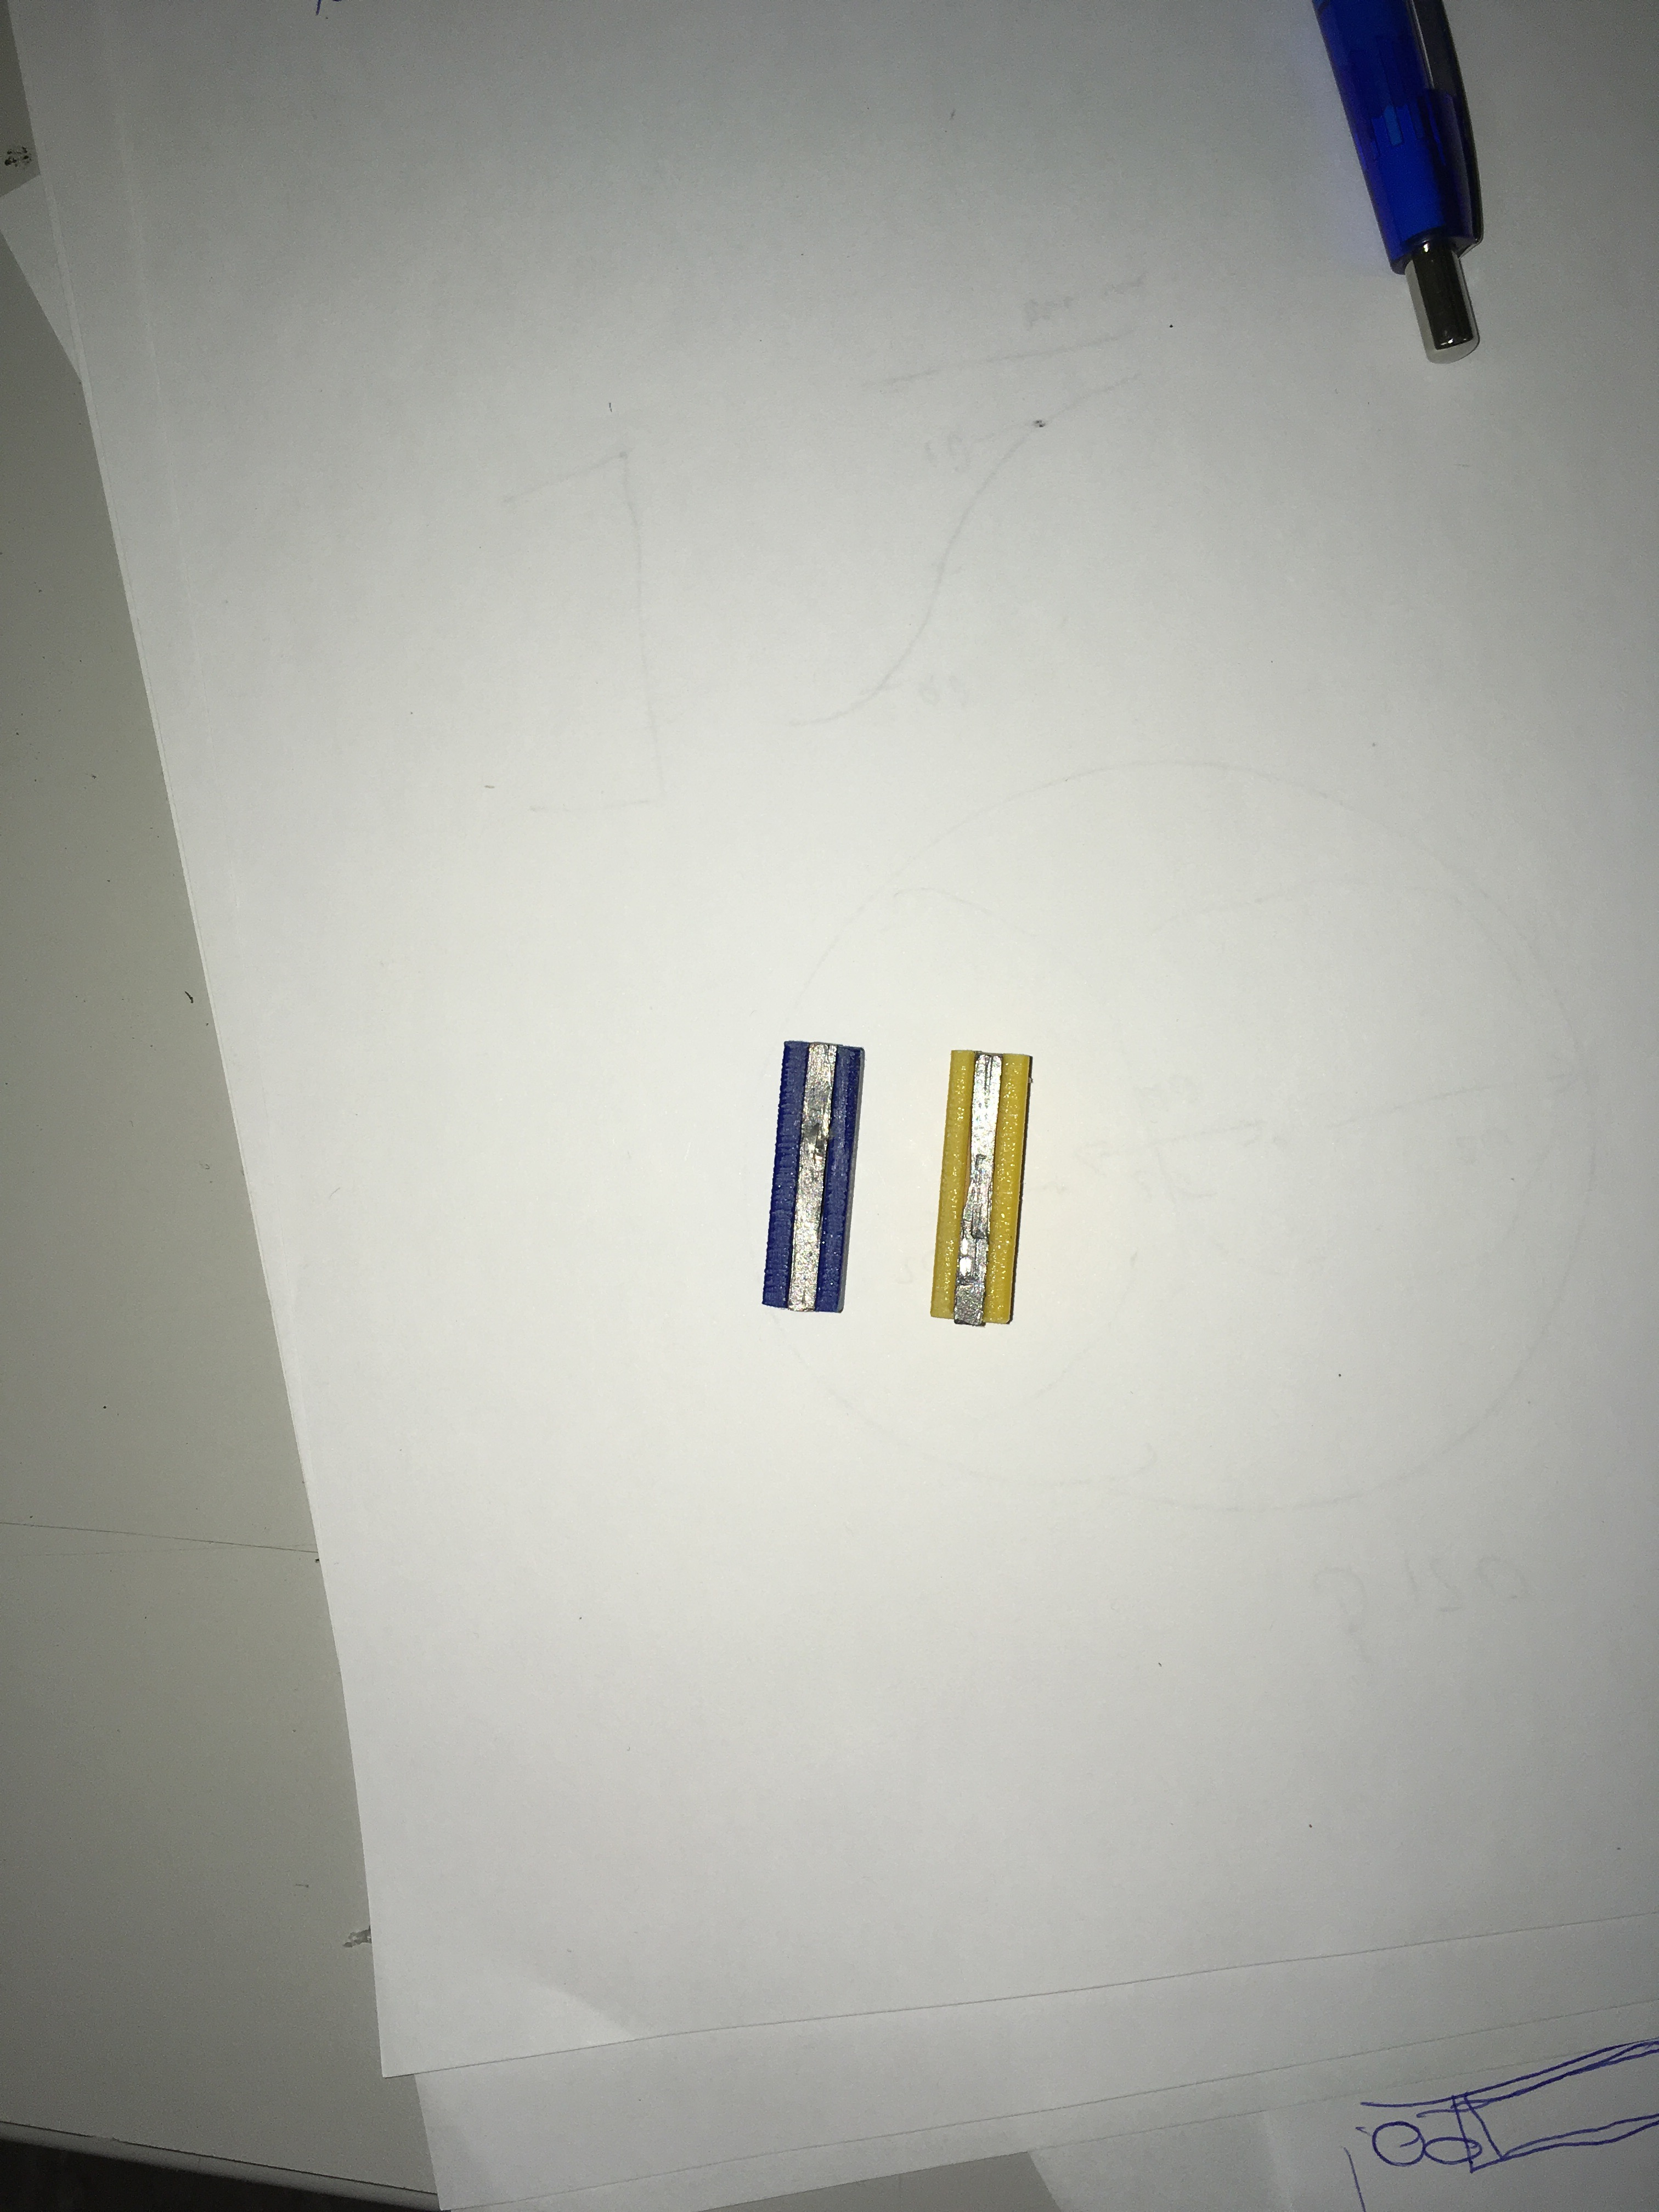
\includegraphics[width=4cm,angle=90]{plots/LeadStrips}
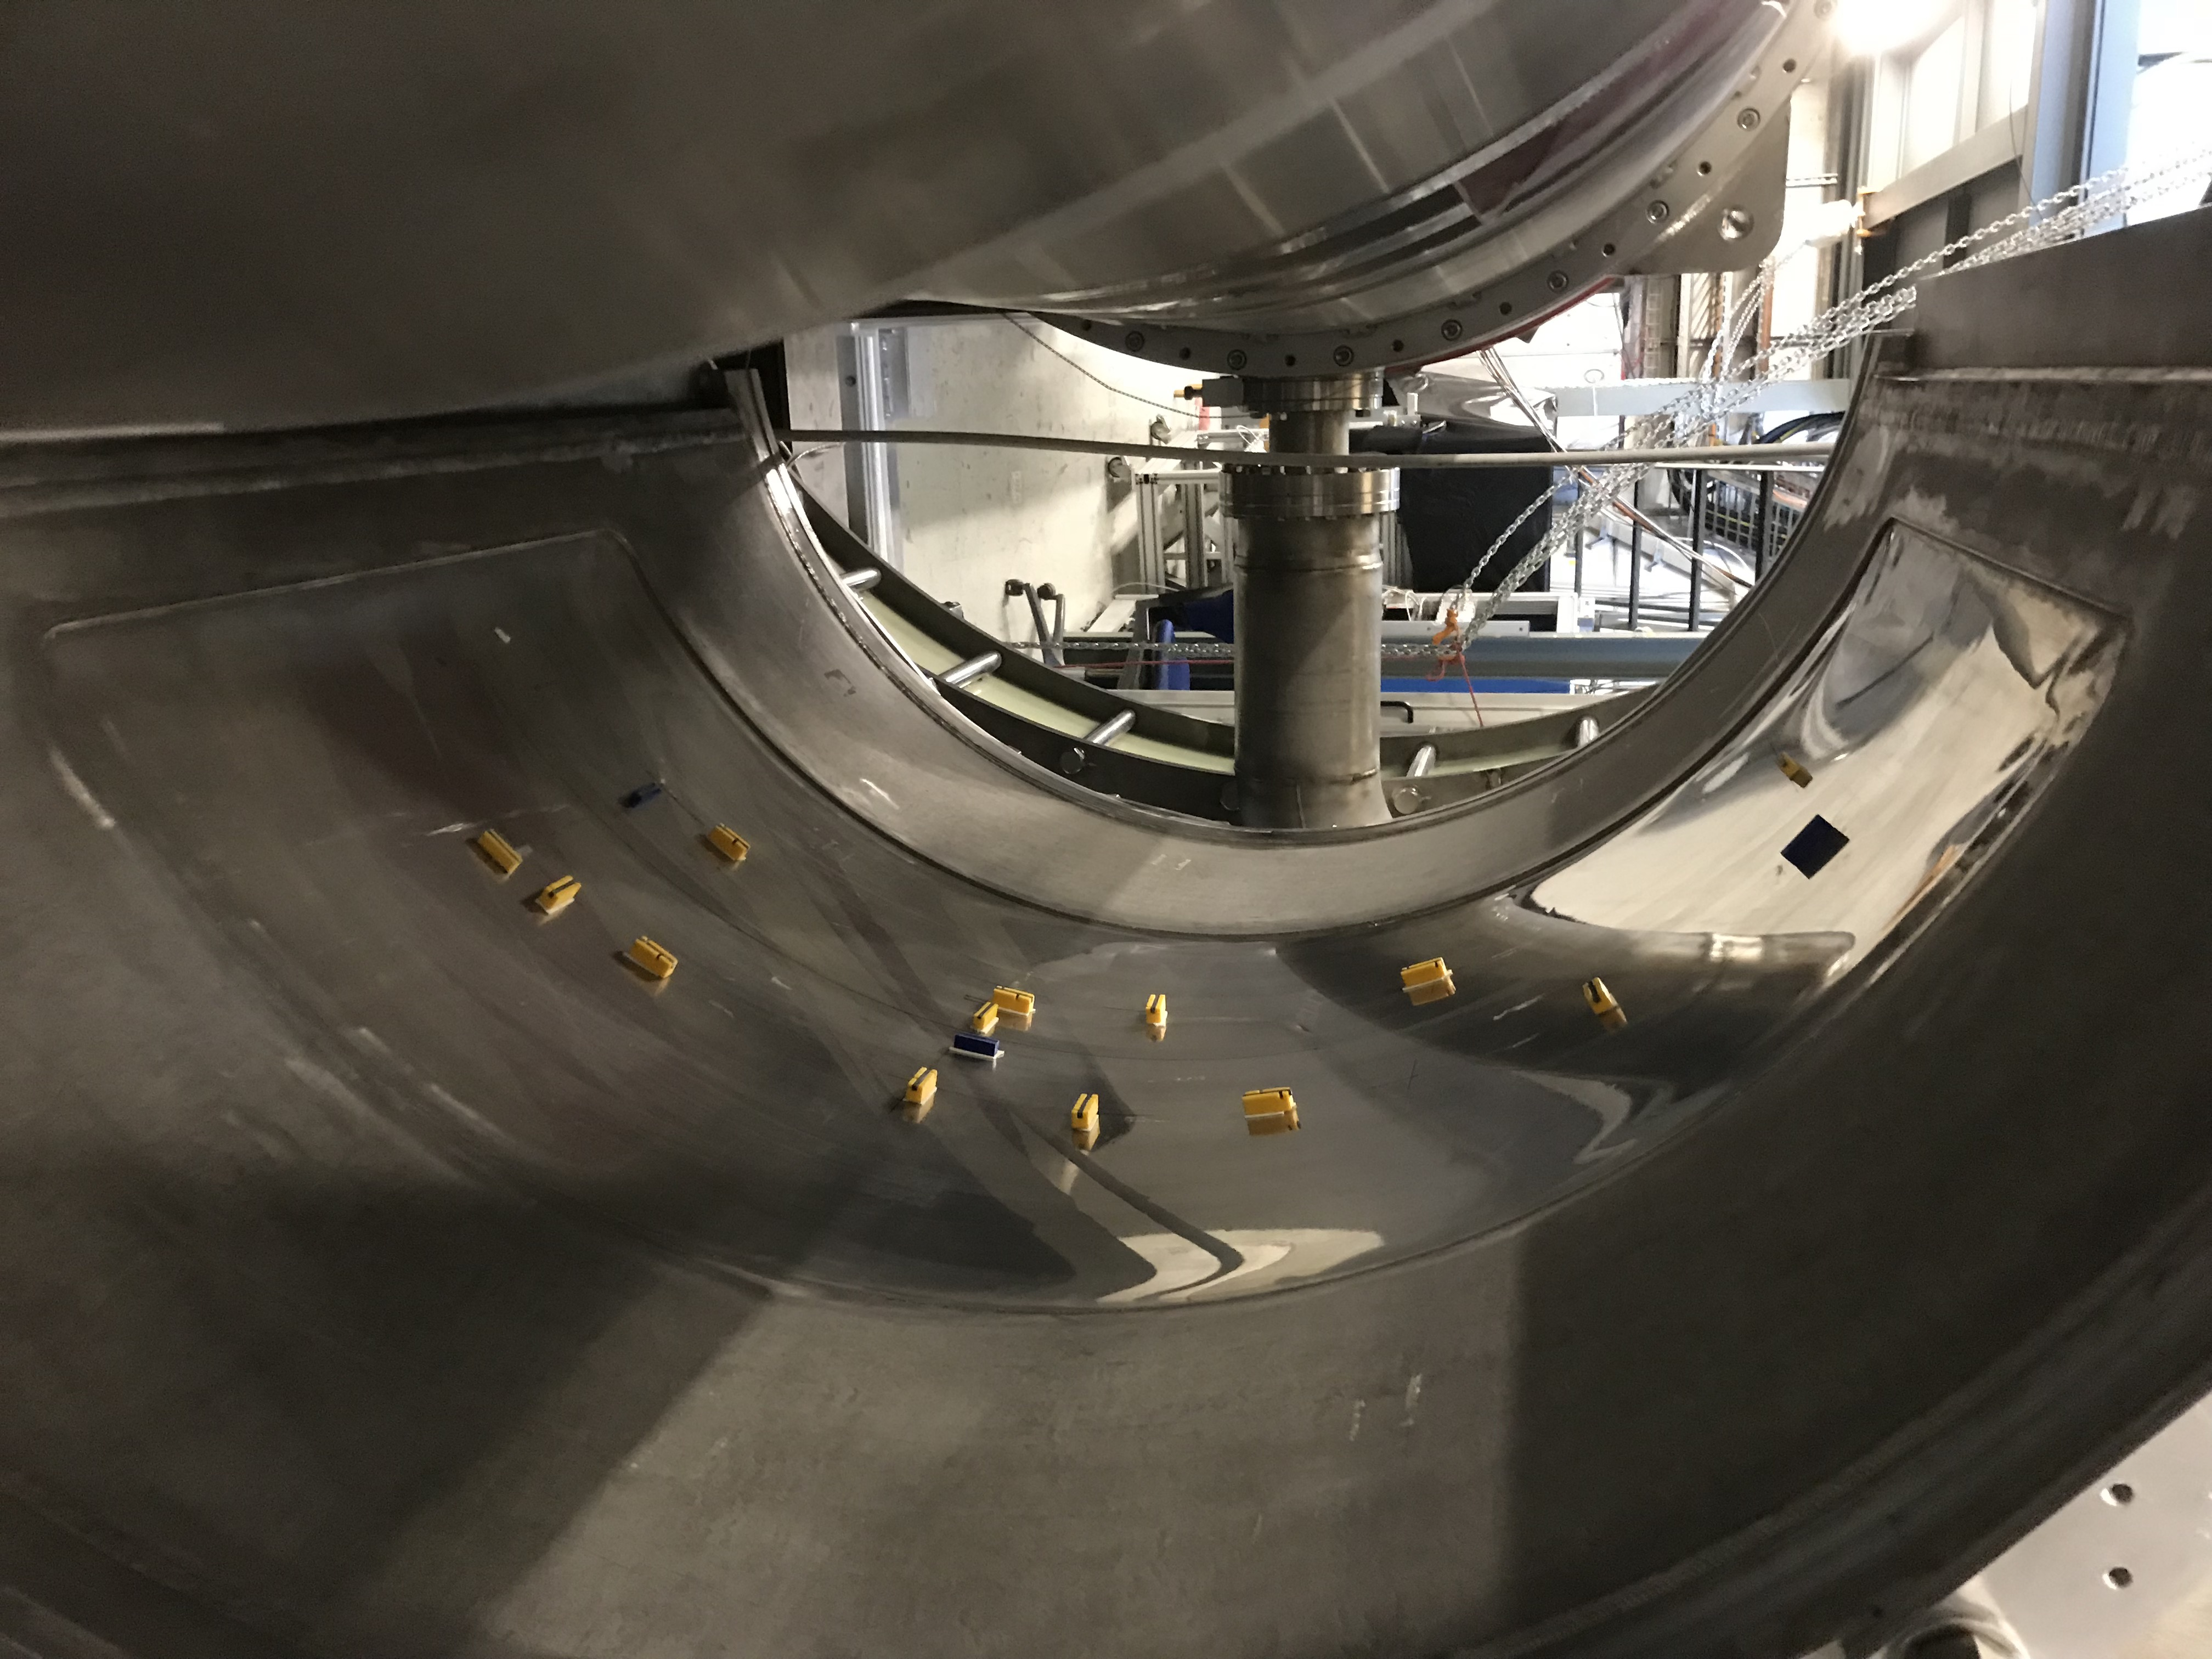
\includegraphics[width=4cm,angle=90]{plots/MountedLeadStrips}
\caption{Lead absorber strips mounted on the inner face
of LXe cryostat. [change lead strip photo]}
\label{fig:lead1} 
\end{figure}
\begin{figure}[]
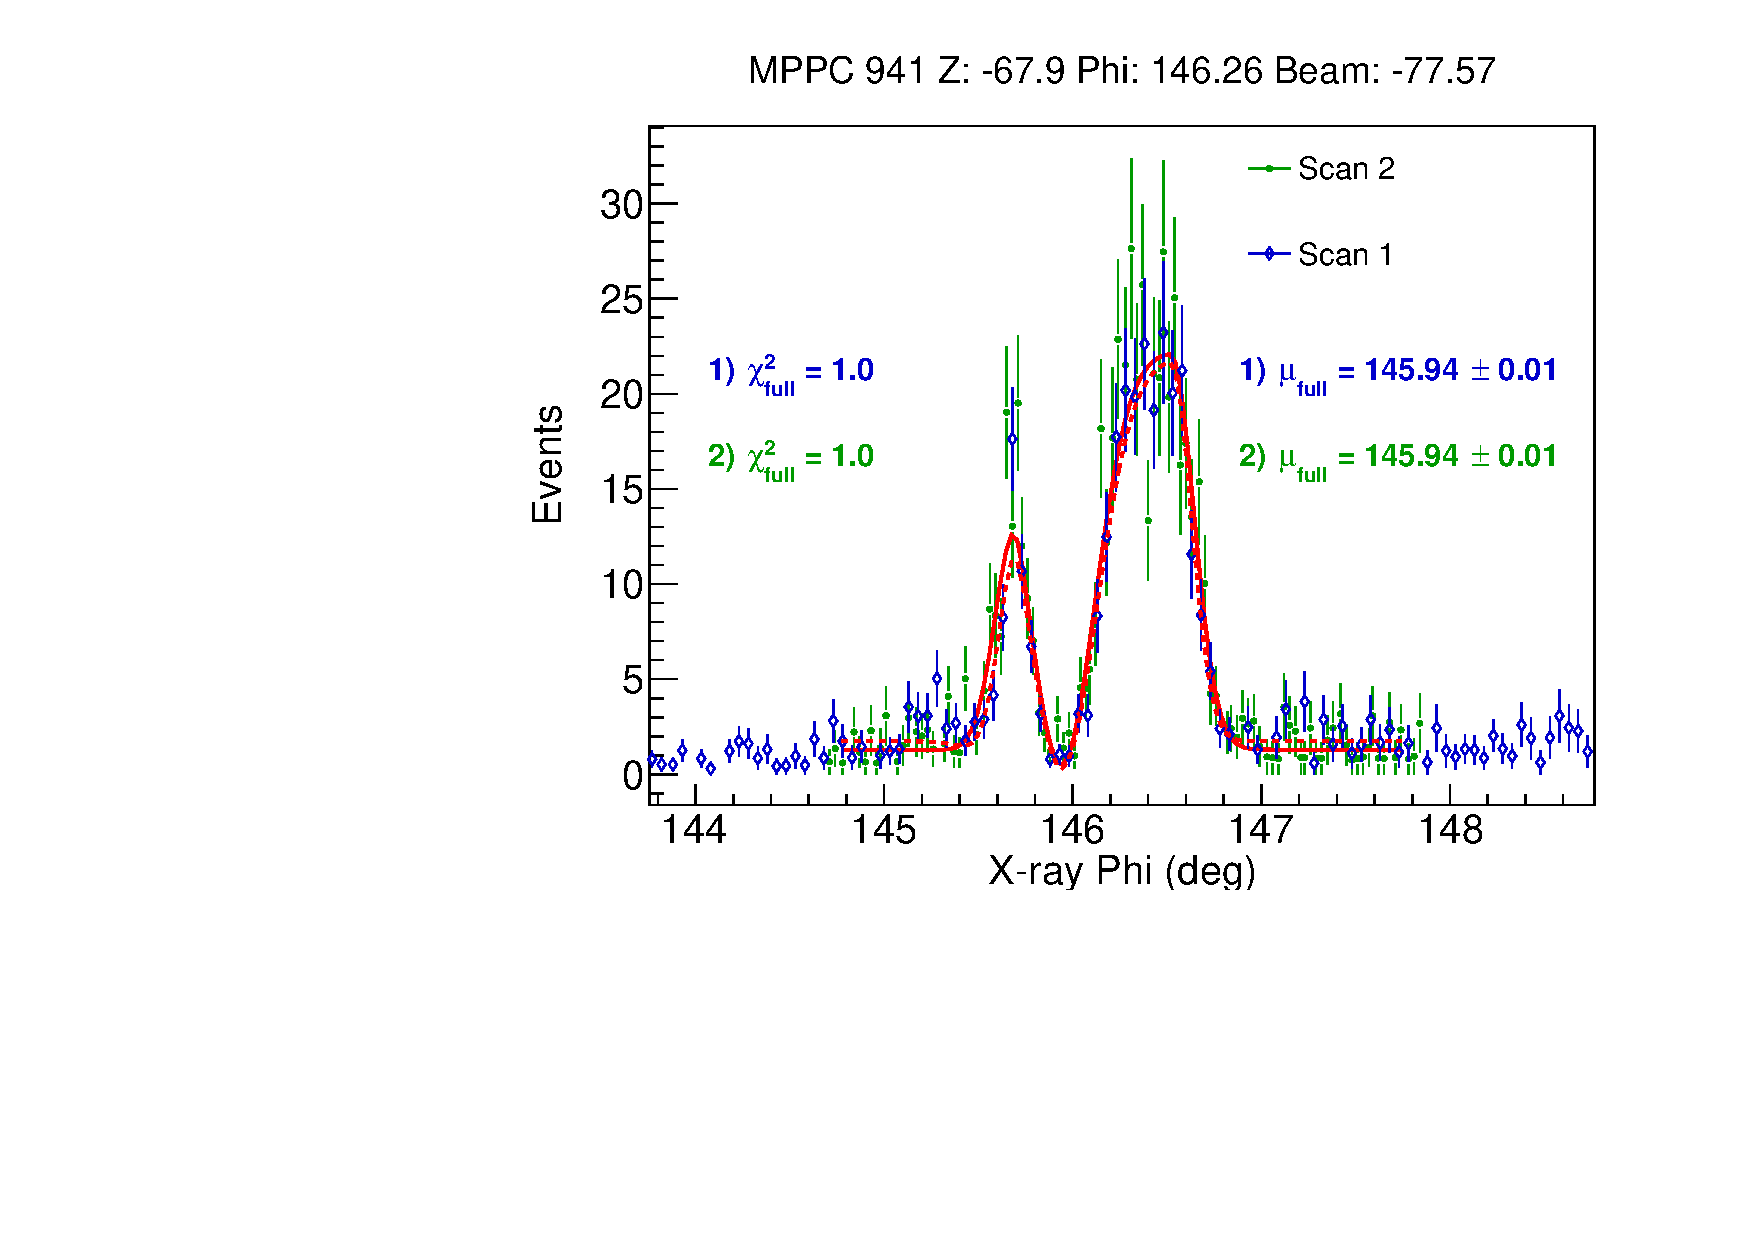
\includegraphics[width=4cm]{plots/2018/c941}
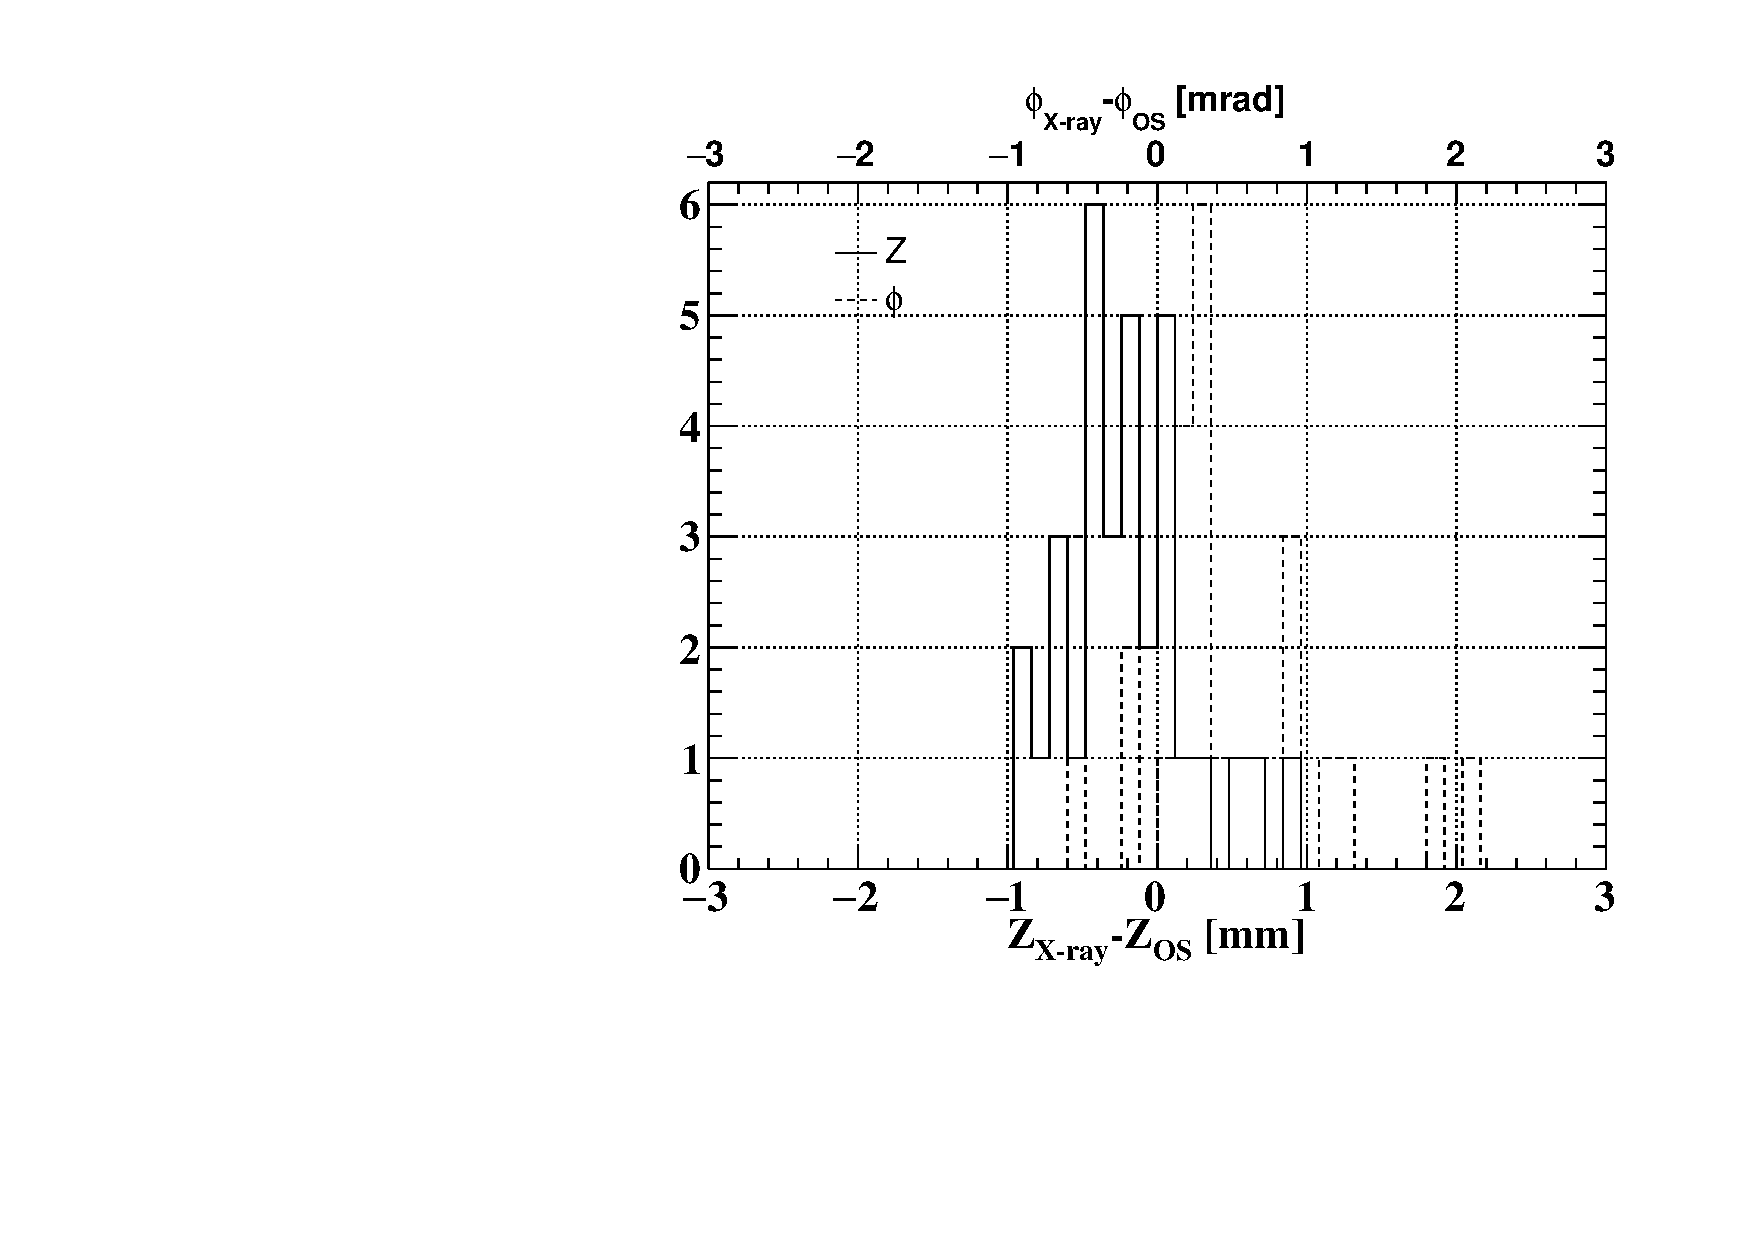
\includegraphics[width=4cm]{plots/2018/dzdphi_lead}
\caption{X-ray event rate recorded by a photodetector 
with reduction of events (shadow) due to the lead absorber strip
(left). The  comparison between strip positions calculated
with X-ray and optical surveys (right). }
\label{fig:lead2} 
\end{figure}

